The closed fuel cycle is one that includes the recycling of used, or spent, fuel
to be reused in a reactor. Recycling used nuclear fuel is expensive due to the
costs associated with handling highly radioactive material (e.g., capital costs
of hot cells, etc.). However, there are at least two overarching benefits that
contribute to lowering the overall cost of the fuel cycle: increasing repository
capacity and increasing fuel utilization.

Spent fuel that exits the average light water reactor (LWR) has an approximate
composition as shown in Table \ref{tab:lwr_fuel}. Of the elements that comprise
used fuel, uranium, plutonium, and the mixed actinides (MA) are all capable of
producing power through the fission process. The fission products, however,
contain isotopes with high neutron capture cross sections, which therefore act
as poisons to the nuclear chain reaction. Achieving theoretical 100\% fuel
utilization would thus require storing indefinitely only the fission products
and any other byproducts of the fuel cycle, rather than additionally having to
store other elemental groups produced by nuclear fission, e.g., minor
actinides. Furthermore, repository capacity is determined not only by total mass
or volume, but also by heat load and radiotoxicity, making the concentration of
high-activity isotopes one of the limiting factors in a repository's
capacity. Fission products are generally short-lived (in comparison to
transuranic elements, i.e., uranium, plutonium, and the MAs). Accordingly, for
repositories with long-term heat load limited capacities, minimizing the amount
of transuranics increases the amount of material that can be stored in a given
repository.

\begin{table} [h]
\centering
\begin{tabular} {|c|c|} 
\hline
Element Group & wt \% \\
\hline
Uranium           & $\sim$95  \\
Plutonium         & $\sim$1   \\
Mixed Actinides   & $\sim$0.1 \\
Fission Products  & $\sim$4   \\
\hline
\end{tabular}
\caption{Elemental Breakdown of Spent Fuel Exiting a Typical LWR}
\label{tab:lwr_fuel}
\end{table}

The act of reprocessing spent fuel is comprised of a number of
subprocesses. Once fuel has left the reactor core, it is stored in a spent fuel
pool for a some number of years, typically around five, in order to provide
enough time to lower decay heat to acceptable levels for handling of the
fuel. It can then be directly sent to a reprocessing facility or be sent for
some period of time to dry-cask storage. Reprocessing nuclear fuel is a chemical
extraction process and therefore is limited by chemical extraction
techniques. In general, there are two types of such processes: low-temperature
methods using organic solvents (e.g., PUREX), and high-temperature methods using
molten salts and metals, called pyroprocessing. The extraction techniques
separate the spent fuel into chemically-similar groups which can vary based on
the technique used, but generally align with those shown in Table
\ref{tab:lwr_fuel}. The separated streams are then sent either to a repository
as high-level waste (HLW) or to an appropriate fuel fabrication
facility. Graphically, the closed fuel cycle is shown in Figure
\ref{fig:closed-cycle}.

\begin{figure}[]
  \begin{center}
    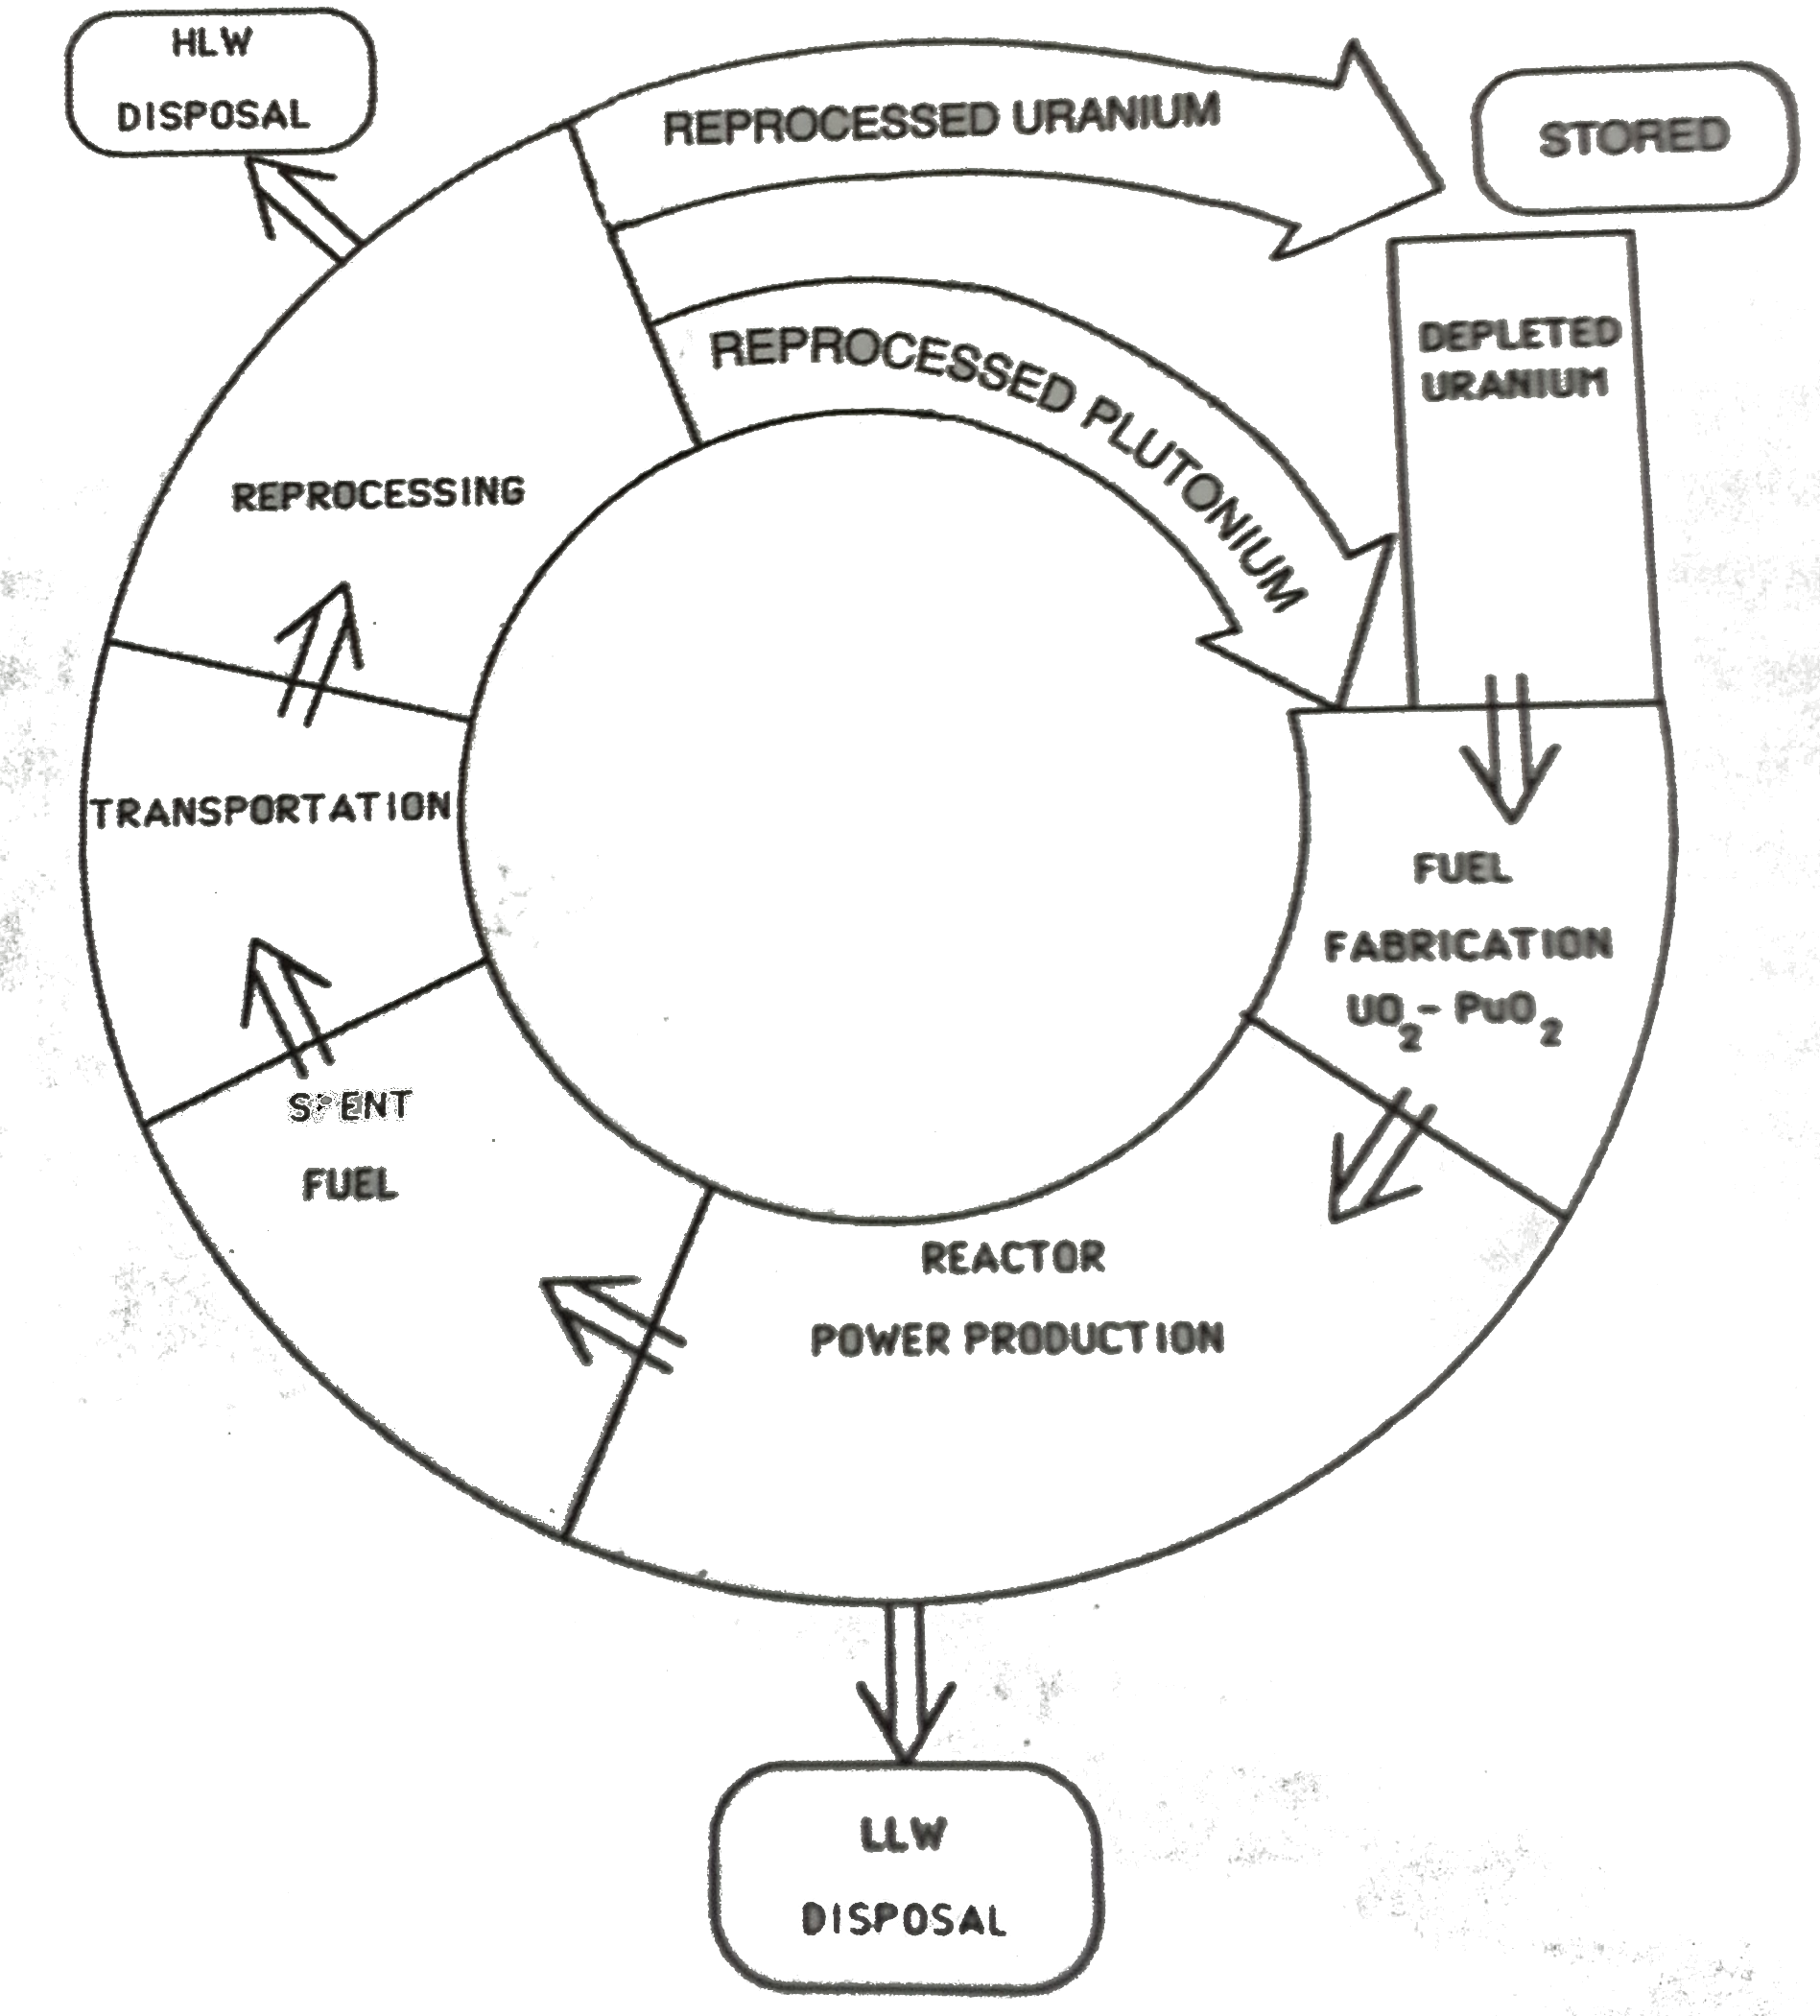
\includegraphics[height=7.5cm]{./chapters/intro/closed_cycle.png}
  \caption{The closed fuel cycle as shown in \cite{cochran1990nuclear}.}
  \label{fig:closed-cycle}
  \end{center}
\end{figure}


The elemental groups used in fuel fabrication will depend on the fuel cycle that
is developed. The currently-operating large-scale industrial reprocessing plants
(La Hague in France, THORP in the U.K., Mayak in Russia, and Rokkasho in Japan)
utilize the PUREX process to extract uranium and plutonium. The plutonium is
then oxidized and mixed with depleted uranium from the enrichment process to
produce mixed-oxide fuel (MOX). Other sources of uranium can be used to fill MOX
fuel, such as recycled uranium from reprocessing, as neutronics-related
reactivity and safety constraints allow. Other fuel cycles utilize the mixed
actinides elemental group as well. Generally, plutonium is included with the
mixed actinides, which results in a elemental category called the transuranic
(TRU) elements. These fuel cycles generally include fast reactors that convert
their TRU inventory into either more TRU (i.e., they have a conversion ratio
(CR) of greater than 1), less TRU (CR < 1), or they maintain the amount of TRU
entering and exiting their system (CR = 1). Fast reactors with CR > 1 are termed
breeder reactors.

It should be noted that with any reprocessing capability, nonproliferation
issues arise. Nuclear weapons have historically been produced using either
enriched uranium or reprocessed plutonium; however it is possible to produce one
with any mix of appropriate materials. Accordingly, any fuel cycle that exposes
bare plutonium streams has an inherently higher nonproliferation risk than one
that does not, and such risks must be weighed accordingly. However, the primary
nuclide that drive such plutonium-based weapons is \nucl{239}{Pu}. Additional
isotopes, e.g., \nucl{240}{Pu}, are considered ``impurities'' that dilute the
efficacy and reliability of plutonium-based weapons. In general, fuel exiting a
full LWR cycle have very poor plutonium profiles for the purpose of weapon
utilization.
